\documentclass[12pt,a4paper]{report}

\usepackage[utf8]{inputenc}
\usepackage[english]{babel}
\usepackage{amsmath}
\usepackage{amsfonts}
\usepackage{amssymb}
\usepackage{graphicx}
\usepackage{hyperref}
\usepackage{todonotes}
\usepackage{xcolor}
\usepackage{listings}
\usepackage{authblk}
\usepackage{algorithm, algpseudocode}
\usepackage{geometry}
\usepackage{booktabs} 
\usepackage{longtable} 
\usepackage{array}
\usepackage{geometry}
\usepackage{tikz}
\usepackage{caption} 

\renewcommand{\lstlistingname}{Example}
\newcommand{\ie}{\textit{i.e.}}
\newcommand{\vnnlib}{VNN-LIB}

%customized todo
\definecolor{lightgreen}{rgb}{0.8,1.0,0.8}
\definecolor{red}{rgb}{0.8,0,0}
\definecolor{green}{rgb}{0,0.8,0}
\definecolor{blue}{rgb}{0,0,1}
% Define some colors for listings
\definecolor{codegreen}{rgb}{0,0.6,0}
\definecolor{codegray}{rgb}{0.5,0.5,0.5}
\definecolor{codepurple}{rgb}{0.58,0,0.82}
\definecolor{backcolour}{rgb}{0.95,0.95,0.92}
\definecolor{keywordblue}{rgb}{0.13,0.13,1}
\definecolor{stringred}{rgb}{0.8,0,0}

% Listings style for BNFC commands
\lstdefinestyle{lbnf}{
    backgroundcolor=\color{backcolour},   
    commentstyle=\color{codegreen},
    keywordstyle=\color{keywordblue}\bfseries,
    numberstyle=\tiny\color{codegray},
    stringstyle=\color{stringred},
    basicstyle=\ttfamily\footnotesize,
    breakatwhitespace=false,         
    breaklines=true,                 
    captionpos=b,                    
    keepspaces=true,                 
    numbers=left,                    
    numbersep=5pt,                  
    showspaces=false,                
    showstringspaces=false,
    showtabs=false,                  
    tabsize=1,
    frame=lines,
    xleftmargin=2em,
    framexleftmargin=1.5em,
    escapeinside={\%*}{*} 
}

% Listings style for Bash/CLI commands
\lstdefinestyle{bash}{
    backgroundcolor=\color{backcolour},   
    commentstyle=\color{codegreen},
    keywordstyle=\color{keywordblue}\bfseries,
    numberstyle=\tiny\color{codegray},
    stringstyle=\color{stringred},
    basicstyle=\ttfamily\footnotesize,
    breakatwhitespace=false,         
    breaklines=true,                 
    captionpos=b,                    
    keepspaces=true,                 
    numbers=left,                    
    numbersep=5pt,                  
    showspaces=false,                
    showstringspaces=false,
    showtabs=false,                  
    tabsize=2,
    frame=lines,
    xleftmargin=2em,
    framexleftmargin=1.5em,
    escapeinside={\%*}{*} 
}

\newcommand{\mytodo}[1]{\todo[inline,color=lightgreen]{TODO:#1}}
\newcommand{\mnote}[2][]{\todo[inline,color=blue!10,#1]{Matthew: #2}}
\newcommand{\myremark}[1]{\todo[inline, color=lightgreen]{\textbf{Remark:} #1}}

\title{
	The \vnnlib{} Standard \\ 
	Version 2.0 (draft)
}

\author[1]{Stefano Demarchi}
\author[2]{Dario Guidotti}
\author[2]{Luca Pulina}
\author[1]{Armando Tacchella}

\author[3]{Ann Roy}
\author[3]{Allen Antony}
\author[3]{Matthew Daggitt}

\affil[1]{University of Genoa, Viale Causa 13, 16145 Genoa, Italy}
\affil[2]{University of Sassari, Via Roma 151, 07100 Sassari, Italy}
\affil[3]{University of Western Australia, 35 Stirling Hwy, Crawley WA 6009, Australia}
  
\begin{document}

\maketitle

\begin{abstract}
This document presents \vnnlib{}, a standard that formalises the query language for neural network verifiers. The standard uses the 
Open Neural Network Exchange (ONNX) format for model description and builds upon the Satisfiability Modulo Theories Library (SMT-LIB) 
format for query specification. Key among the standard is a formally defined syntax and semantics, complimentary tooling, as well as a 
command-line interface for verifiers. The goal is to foster greater robustness and interoperability in the neural network verification 
landscape.
\end{abstract}

\chapter{Introduction}
\label{sec:intro}

\section{Motivation}

While neural networks have shown exceptional performance across a range of tasks, 
they remain vulnerable to issues such as adversarial examples~\cite{szegedy2013intriguing} and discriminatory behaviour~\cite{4}. As these models are increasingly deployed in safety-critical and high-impact societal applications~\cite{1,2,3}, the need for robust methods to verify their behaviour has become paramount.

As with many formal verification problems, neural network verification can typically be reduced to sets of satisfiability queries. These queries are answerable by domain specific solvers which will be referred to as \emph{neural network verifiers} or simply \emph{verifiers} in this document. The \vnnlib{} standard was inspired by the success of SMT-LIB, which provides a unified format for queries to SMT solvers. 
Since its introduction in 2023, the \vnnlib{} standard~\cite{5} has been the de-facto specification language for queries in the neural network verification community, most notably used in the annual VNN-COMP~\cite{7} competition. Its goal is to facilitate the standardisation of solver interfaces and enable the collection of neural network verification benchmarks in a common format. 

\section{Document structure}

This document assumes some basic familiarity with neural networks, first-order logic and simple type theory. The document is orgnaised as follows:
\begin{enumerate}
\item \textbf{Chapter~\ref{sec:models} - \nameref{sec:models}}: A high-level description of the pre-existing ONNX standard for representing the neural network models.
\item \textbf{Chapter~\ref{sec:specification_language} - \nameref{sec:specification_language}}: The \vnnlib{} language for representing a satisfiability query over one or more neural network models.
\item \textbf{Chapter~\ref{sec:theories-logics} - \nameref{sec:theories-logics}}: A system for describing the different subsets of the query language that a given solver may support.
\item \textbf{Chapter~\ref{sec:solver_interface} - \nameref{sec:solver_interface}}: A standardised interface for allowing users to invoke a neural network verifier on a query and to query the capabilities of the verifier.
\end{enumerate}

\section{Document versioning}

New versions of the document are identified by semantic versioning. In general patch versions will fix bugs in the document, minor versions will include conservative extensions to the specification, while changes to the major version number will result from major backwards-incompatible changes.

\subsection*{Changelog for v2.0}

\paragraph{Authors:} Allen Antony, Ann Roy, Matthew Daggitt with regular input from Stefano Demarchi, Andrea Gimelli.

\noindent \paragraph{Acknowledgements:} This version of the standard was developed with the help of many others in the neural network verification community.
Particular thanks must given to the following people, who provided many helpful suggestions, constructive criticism and encouragement: Taylor Johnson, Samuel Teuber, Wen Kokke, Julien Girard, Guilhem Ardouin, Augustin Lemesle, Michele Alberti, Julien Lehmann, Thomas Flinkow, Edoardo Manino, Omri Isac, Guy Katz, Idan Refaeli, David Shriver and Christopher Brix.

\noindent \paragraph{Changes from previous version:}
\begin{itemize}
\item Formal grammar for query language
\item Added explicit network declarations to the query language.
\item Add support for networks with multiple inputs/outputs and hidden layers.
\item Added support for multiple networks
\item Added a formal type system and semantics.
\item Added theories and logics.
\item Introduction of the command-line interface: \texttt{verify} and \texttt{supports}.
\end{itemize}

\subsection*{Changelog for v1.0}

\paragraph{Authors:} Stefano Demarchi, Dario Guidotti, Luca Pulina, Armando Tacchella

\paragraph{Contents:}
\begin{itemize}
\item Initial release.
\item Outline of goal
\item Proposal of initial syntax of the query language.
\end{itemize}

\chapter{Network Models}
\label{sec:model}

\section{Introduction}
\label{sec:model_intro}
At a high level, networks can be seen as functions 
$\nu : I^n \to O^m$, mapping one or more $n$-dimensional \emph{input domains}
$I^n$ ($n > 0$) to one or more $m$-dimensional \emph{output domains} $O^m$ ($m>0$). 
We argue that this representation captures most cases of practical
interest.

For instance, a network computing an approximation
of some function $f: \mathbb{R}^n \to \mathbb{R}$ would have $I = O =
\mathbb{R}$, whereas a network classifying 8-bit images of size $h \times v$ in
two classes would be defined as ${\nu: \{0,\ldots,255\}^{h \cdot v}
\to \{0, 1\}}$ with $I=\{0, \ldots, 255\}$ and $O = \{0,1\}$.

At a lower level, neural networks can be described as a computational graph, specifically a directed acyclic graph (DAG), where nodes represent operations 
(e.g., addition, multiplication, activation functions) and edges represent the flow of data (tensors) between these operations. The DAG receives (one or more) input tensors, 
processes them through a series of operations, and produces (one or more) output tensors.

\section{Network Formats}
\label{sec:model_formats}
Neural networks are represented in serialized formats that allow for model saving, sharing, and deployment. Framework-native formats (e.g., TensorFlow's .ckpt, PyTorch's .pth) are 
designed for integration with a single deployment environment, while interoperable formats are developed to facilitate cross-framework compatibility. 

\subsection{Interoperable Network Formats}
Interoperable formats are designed to allow neural networks to be shared and executed across different frameworks and hardware platforms. Some of the most notable formats include:
\begin{itemize}
	\item \textbf{ONNX (Open Neural Network Exchange)}: A widely adopted format that supports a variety of neural network architectures and operations, enabling models to be shared across different frameworks.
	\item \textbf{NNEF (Neural Network Exchange Format)}: A format developed by the Khronos Group, designed for efficient deployment of neural networks across different hardware platforms.
	\item \textbf{Safetensors}: A format that ensures the security and integrity of neural network models, preventing tampering and ensuring safe loading.
	\item \textbf{GGUF}: A format originating from the Llama project, which is designed for efficient execution of quantised models on low-power hardware. 
\end{itemize}

\subsection{Justification for ONNX}
ONNX is chosen as the standard format for \vnnlib{} for several reasons:
\begin{itemize}
	\item \textbf{Widespread Industry Adoption}: ONNX conversion is supported by frameworks such as PyTorch, and Tensorflow, making it ideal for framework-agnostic model representation.
	\item \textbf{Rich Operator Set}: ONNX supports a wide range of operators, enabling the representation of complex neural network architectures.
	\item \textbf{Neural Network Verification Adoption}: ONNX has an established presence in NNV research, since VNN-COMP has used ONNX as the standard format for benchmarks.
	\item \textbf{Rigorous Specification}: ONNX models are rigorously specified computation graphs with strongly-typed data tensors and versioned (via opsets) operators, eliminating ambiguity.
\end{itemize}

\section{ONNX Format Overview}
\label{sec:onnx_overview}
ONNX is a standardized format for representing neural networks as directed acyclic graphs (DAGs). An ONNX model is serialized into a single binary file (with a .onnx extension) using Google's Protocol Buffers 
(Protobuf), a language and platform-neutral mechanism for serializing structured data

\subsection{ONNX Model Structure}
The ONNX model \texttt{GraphProto} contains the following key components:
\begin{itemize}
	\item \textbf{Node}: Each node has an operation (e.g., convolution, activation), a type (e.g., Conv, Relu) and attributes 
	(e.g., kernel size, stride), and contains a list of inputs and outputs, representing the tensors that flow into and out of the operation.
	\item \textbf{Initializer}: These are tensors that are used as constants in the model, such as weights and biases.
	\item \textbf{Metadata}: This describes attributes of the model such as model version, author, and description.
	\item \textbf{Input/Output}: These specify the external inputs and outputs of the model, including their names, datatypes, and shapes.
\end{itemize}

\subsection{ONNX Tensors}
Data within ONNX models is strongly typed, with each tensor having a specific numeric type and shape. The supported properties for a tensor include:
\begin{itemize}
	\item \textbf{Element Type}: ONNX defines a standard set of numeric types \href{https://onnx.ai/onnx/intro/concepts.html#element-type}{here}. 
	The most commonly used types for neural network verification are: 32-bit floating point (FLOAT), and 16-bit floating point (FLOAT16). Signed and unsigned integers (e.g., INT32, UINT8) are also supported, 
	but less common in neural networks.
	\item \textbf{Shape}: The shape of a tensor is defined as a list of integers, where each integer represents the size of the corresponding dimension. For example, a tensor with shape [3, 224, 224] 
	represents an image with 3 color channels (RGB) and dimensions 224x224 pixels.
	\item \textbf{Values}: A contiguous block of memory containing data of a specific numeric type.
\end{itemize}

\subsection{ONNX Opsets}
ONNX uses a versioning system called \emph{opsets} to manage the evolution of operators. Each operator is associated with a specific opset version, which defines its semantics and attributes.
This ensures that the precise mathematical definition and behaviour of each operator is well-defined and can evolve over time without breaking existing models. The ONNX model file declares the opset
version used.
	
\section{\vnnlib{} Support for ONNX}
\label{sec:onnx_support}
\vnnlib{} supports query specification for any abritary ONNX model that is sequential. In practice however, most verifiers support a subset of ONNX operators and datatypes. Additionally, verifiers may not support
models with multiple inputs and/or outputs. To ensure clarity, transparency, and interoperability, \vnnlib{} defines as part of its verifier interface (Section~\ref{sec:solver_interface}), a capability query 
mechanism that allows users to determine the ONNX operators, datatypes, and model structures supported by a specific verifier. This is detailed in Section~\ref{sec:global_capabilities}.

\section{ONNX Operators}
\label{sec:supported_operators}
The following operators cover almost every benchmark provided in the
VNN-COMP repositories for sequential networks; other kinds of networks
(ResNet, Recurrent, etc.) are often based on ``exotic'' and, in general,
peculiar operators that do not lie in this list.

\begin{itemize}
	\item \emph{Add (Add)} operator performs the element-wise sum of
		a tensor and a scalar. We strongly encourage to use the 
		\textit{Gemm} operator when paired with \textit{MatMul}.
	
	\item \emph{AveragePool (Average Pooling)} operator
	  supports downsampling with averaging.
	
	\item \emph{BatchNormalization (Batch
	  Normalization)} operator supports adjusting and scaling the
	  activations functions, and it is expressive enough to represent
	  general batch normalization.
	  
	\item \emph{Concat (Concatenation)} operator concatenates a list
		of tensors into a single tensor, with the same shape except for
		the axis to concatenate on.	
	
	\item \emph{Conv (Convolutional)} operator supports
	  all the attributes to encode a generic convolutional layer.
	
	\item \emph{Dropout (Dropout)} operator supports
	  random dropping of units (during training). This operator should not
	  appear on trained models.  
	  
	\item \emph{Flatten (Flatten)} this operator converts multidimensional
	  arrays (tensors) to single dimensional ones; it is used instead of
	  \emph{Reshape} in some of the models in the zoo.
	  
	\item \emph{Gemm (General Matrix Multiplication)}
	  operator encodes matrix multiplication possibly with a scalar
	  coefficient and the addition of another matrix; as such \emph{Gemm}
	  can encode fully connected layers in neural networks.
	
	\item \emph{LRN (Local Response Normalization)}
	  operator supports normalization over local input regions; it is uatilized
	  in Alexnet and derived networks.
	  
	\item \emph{MatMul (Matrix Multiplication)} operator performs a
		numPy-like matrix multiplication. We strongly encourage to use
		the \textit{Gemm} operator.
	  
	\item \emph{MaxPool (Maximum pooling)} operator supports
	  downsampling with maximization.
	
	\item \emph{ReLU (Rectified Linear Unit)} operator
	  encodes the corresponding activation function $\sigma(x) = \max(0, x)$.
	  
	\item \emph{Reshape (Reshape)} operator supports
	  reshaping of the tensor's dimensions.
	  
	\item \emph{Sigmoid (Logistic Unit)} operator
	  encodes the corresponding activation function $\sigma(x) =
	  \frac{1}{1 + e^{-x}}$.
	  
	\item \emph{SoftMax (Softmax Unit)} operator transforms
	  vectors into probabilities, e.g., for selecting among different
	  classes and it is commonly utilized in state of the art
	  networks.
	  
	\item \emph{Sub (Sub)} operator performs element-wise binary subtraction
		between two tensors.
	
	\item \emph{Unsqueeze (Unsqueeze)} operator removes dimensions of size
	  1 from tensors, and it is utilized, e.g., in \emph{Densenet} and
	  \emph{Inception2}.
\end{itemize}




\chapter{Query Language}\label{sec:specification_language}

The SMT-LIB language is a well-known language used to formalize 
Satisfiability Modulo Theories problems, and is expressive enough to
represent the verification properties of interest. In this language, 
it is possible to define both the \textit{pre-} and 
\textit{post-}conditions at once, by defining the variables for the
input and the output of the neural network. In the following we
show some examples of networks and corresponding properties in the
SMT-LIB language.

\section{Syntax}
\label{sec:syntax}

The syntax of VNN-LIB is formally defined using Labelled Backus-Naur Form (LBNF)\cite{8}. LBNF is a variant of BNF that allows for 
annotations (labels) on productions, facilitating the automatic generation of abstract syntax trees, parsers, and other language processing tools. 
This formal grammar provides a rigorous foundation for the language, eliminating ambiguities present in previous versions and ensuring consistent 
parsing across different tools.

The full LBNF grammar for VNN-LIB is provided in the Appendix~\ref{app:lbnf_grammar}. The following subsections highlight key syntactic constructs of the language,
with examples illustrating their usage.

\subsubsection*{Comments}
Comments in VNN-LIB are denoted by a semicolon (\texttt{;}) and extend to the end of the line. They are used for annotation, explaining logic, or providing additional context.

\subsubsection*{Variable Names}
All variable names follow the same syntax conventions. Variable names in VNN-LIB are case-sensitive, must start with a letter, and may only contain letters, digits and underscores. All variable names must
be unique across the scope of the VNN-LIB query. The \texttt{@} character is a reserved character which is used to denote multiple applications of the same network, for the purpose of defining 
hyperproperties such as monotonicity. For example \texttt{(declare-network acasXu@1 ...)} and \texttt{(declare-network acasXu@2 ...)} define two networks that are both instances of the same ONNX model, 
denoted as \texttt{acasXu} in the command line interface of the verifier (See Chapter~\ref{sec:solver_interface} for more details).

\subsubsection*{Whitespace}
Whitespace in VNN-LIB is used to separate tokens and improve readability. It can include spaces, tabs, and newlines. Whitespace is ignored by the parser, except where it is necessary to separate tokens.

\subsubsection*{Network declarations}
\label{sec:network-declarations}
A network declaration is introduced by the keyword \texttt{declare-network}, followed by a user-defined variable name for the network, 
and then its associated input, hidden, and output variable declarations. All variables are declared inside of network declarations and variable 
names must be unique within the scope of the entire VNN-LIB specification.  The network name (e.g., \texttt{simple\_net} below) is used by the verifier to 
associate the declared network with a specific ONNX file provided via the command line (as described in Chapter~\ref{sec:solver_interface}) while the variable names 
(e.g., \texttt{X}, \texttt{Y}) are used to reference nodes inside of the ONNX graph. Figure~\ref{fig:simple_net} shows a simple network declaration along with its ONNX
model representation.

\begin{figure}[htbp]
    \begin{minipage}[c]{0.55\textwidth}
        \begin{lstlisting}[
            style=lbnf,
            label={lst:network_definition}
        ]
(declare-network simple_net
    (declare-input X Real 1 10)
    (declare-output Y Real 1 2)
) 
        \end{lstlisting}
    \end{minipage}%
    \begin{minipage}[c]{0.45\textwidth}
        \centering
        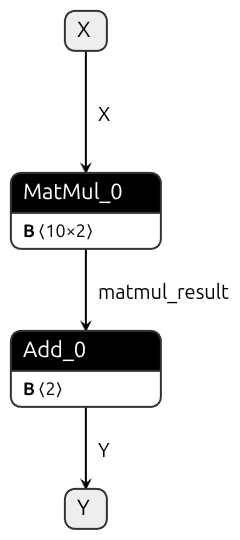
\includegraphics[height=8cm]{imgs/simple_net.onnx.png}
    \end{minipage}
    \caption{A simple VNN-LIB network declaration.}
    \label{fig:simple_net}
\end{figure}

\subsubsection*{Multiple networks}
\label{sec:multi-network-declarations}
VNN-LIB supports defining multiple networks in a single file by including multiple `(declare-network ...)` expressions. This is essential for properties that compare networks, 
such as checking for equivalence between two models or verifying properties of a composite system, like an observer-controller architecture. Figure~\ref{fig:multi_network} 
shows an example of a VNN-LIB file that declares two networks, \texttt{teacher\_net} and \texttt{student\_net}.

\begin{figure}[htbp]
    \begin{minipage}[c]{0.55\textwidth}
        \begin{lstlisting}[
            style=lbnf,
            label={lst:multi_network}
        ]
(declare-network teacher_net
    (declare-input x_teacher Real 1 32)
    (declare-output y_teacher Real 1 2)
)

(declare-network student_net
    (declare-input x_student Real 1 32)
    (declare-output y_student Real 1 2)
)
        \end{lstlisting}
    \end{minipage}
    \begin{minipage}[c]{0.45\textwidth}
        \centering
        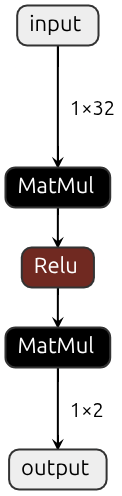
\includegraphics[height=8cm]{imgs/teacher_net.onnx.png}
        \vspace{0.5cm} 
        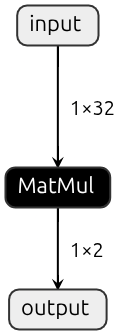
\includegraphics[height=8cm]{imgs/student_net.onnx.png}
    \end{minipage}
    \caption{Two networks declared in VNN-LIB: \texttt{teacher\_net} and \texttt{student\_net}.}
    \label{fig:multi_network}
\end{figure}

\subsubsection*{Input and Output Variable Declarations}
\label{sec:input-output-declarations}
An input variable is declared using the \texttt{declare-input} keyword, followed by a variable name, its element type (e.g., \texttt{Real}, \texttt{int8}), 
and a space-seperated list of integers representing the shape of the tensor. Similarly, an output variable uses the \texttt{declare-output} keyword. Multiple 
input and output variables can be declared within a single network declaration. There are two ways to map these declared variables to the nodes in the ONNX model:
\begin{enumerate}
    \item \textbf{Ordered Mapping (Default):} The variables are mapped to the ONNX graph's inputs/outputs based on their order of declaration. This is demonstrated in Example~\ref{lst:ordered_mapping}
    \item \textbf{Explicit Name Mapping:} Alternatively, variables can be explicitly mapped using its identifier within the ONNX graph. If this method is used, all input and output 
        variables within that network declaration must be given an explicit ONNX node name. This is demonstrated in Example~\ref{lst:named_mapping}.
\end{enumerate}

\begin{figure}[htbp]
    \centering
    \begin{lstlisting}[
        caption={A network with multiple inputs/outputs, mapped by declaration order.},
        style=lbnf,
        label={lst:ordered_mapping}
    ]
(declare-network multi_io_net
    (declare-input image Real 1 3 224 224)
    (declare-input metadata Real 1 10)
    (declare-output logits Real 1 1000)
    (declare-output bbox Real 1 4)
)
    \end{lstlisting}
    \begin{lstlisting}[
        caption={The same network, but with explicit ONNX node name mapping.},
        style=lbnf,
        label={lst:named_mapping}
    ]
(declare-network multi_io_net
    (declare-input image Real 1 3 224 224 onnx-node:"image")
    (declare-input metadata Real 1 10 onnx-node:"metadata")
    (declare-output logits Real 1 1000 onnx-node:"logits")
    (declare-output bbox Real 1 4 onnx-node:"bbox")
)
    \end{lstlisting}
    \vspace{0.5cm}
    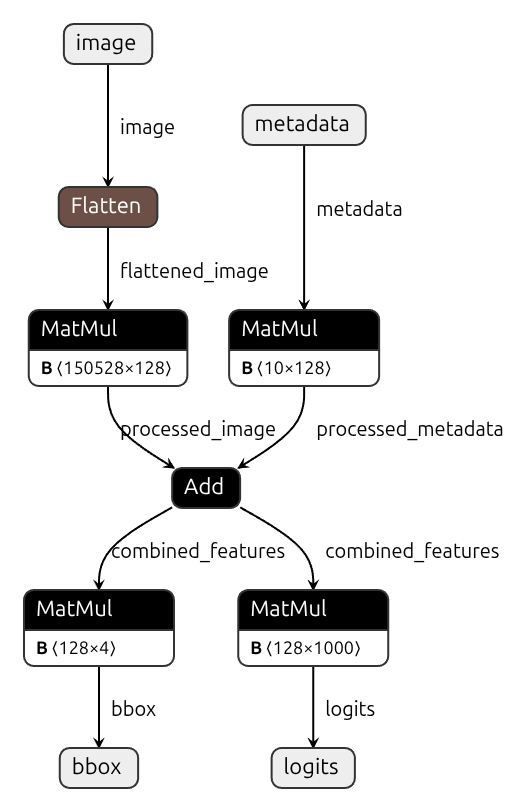
\includegraphics[height=10cm]{imgs/multi_io_net.onnx.png}
    \caption{A VNN-LIB network declaration with multiple inputs and outputs. The first example uses ordered mapping, while the second uses explicit ONNX node names.}
    \label{fig:multi_io_net}
\end{figure}

\subsubsection*{Hidden Node Declarations}
\label{sec:hidden-node-declarations}
A hidden node is declared using the \texttt{declare-hidden} keyword. This declaration includes a variable name for use within the VNN-LIB specification, 
its element type, its tensor shape, and crucially, a string identifier that specifies the corresponding node name in the ONNX graph. The ability to declare hidden nodes
allows for properties to reference key intermediate computations within the network, such as encoding features, attention mechanisms, or other internal states. Multiple
hidden nodes can be trivially declared within a single network declaration. Figure~\ref{fig:hidden_node} shows an example of a VNN-LIB network declaration with a hidden node.

\begin{figure}[htbp]
    \begin{minipage}[c]{0.55\textwidth}
        \begin{lstlisting}[
            style=lbnf,
            label={lst:hidden_node}
        ]
(declare-network encoder
    (declare-input X Real 1 28 28)
    (declare-hidden feature_embedding Real 1 128 onnx-node:"encoder_layer4/output")
    (declare-output Y Real 1 10)
)
        \end{lstlisting}
    \end{minipage}%
    \begin{minipage}[c]{0.45\textwidth}
        \centering
        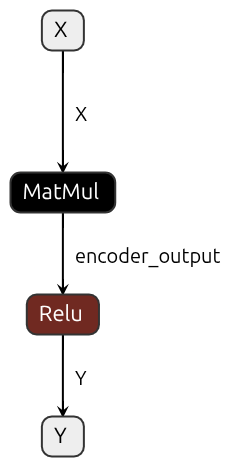
\includegraphics[height=8cm]{imgs/encoder_net.onnx.png}
    \end{minipage}
    \caption{A VNN-LIB network declaration with a hidden node. The hidden node \texttt{feature\_embedding} corresponds to the ONNX node \texttt{encoder\_layer4/output}.}
    \label{fig:hidden_node}
\end{figure}

\subsubsection*{Assertion declarations}
\label{sec:assertion-declarations}
VNN-LIB supports quantifier-free logical formulas as \textit{assertions}. Assertions are defined using parenthesized \texttt{(assert\ldots)} expressions, and following an SMT-LIB-like syntax with the 
operator preceding its operands. An assertion is a logical formula that may include logical connectives, relational comparisons, and arithmetic expressions over declared tensors and constants.

\subsubsection*{Variables and Indexing}
\label{sec:variables-and-indexing}
Assertions may only refer to individual elements of declared tensors. To refer to a specific scalar element within a tensor, an indexing notation is used. Let $X \in I$ be an $n$-dimensional tensor 
in some generic input domain $I = I^{d_1 \times \cdots \times d_n}$. The ``matrix notation'' represents a specific element $x_{i_1, i_2, \dots, i_n}$ of the tensor $X$ as \texttt{X[$i_1$,$i_2$,\dots,$i_n$]}, 
where $i_1, \dots, i_n$ are zero-based indices ranging from $0$ to $d_1{-}1$, $0$ to $d_2{-}1$, \dots, $d_n{-}1$, respectively. To better clarify, if we consider the 1-D tensor $X \in I^n$, the 2-D tensor 
$Y \in I^{n \times m}$, and the 3-D tensor $Z \in I^{n \times m \times p}$, we will have the following representations:
\begin{itemize}
    \item \texttt{X[0]}, \texttt{X[1]}, \dots, \texttt{X[$i$]}, \dots, \texttt{X[$n$]};
    \item \texttt{Y[0,0]}, \texttt{Y[0,1]}, \dots, \texttt{Y[$i$,$j$]}, \dots, \texttt{Y[$n$,$m$]};
    \item \texttt{Z[0,0,0]}, \texttt{Z[0,0,1]}, \dots, \texttt{Z[$i$,$j$,$k$]}, \dots, \texttt{Z[$n$,$m$,$p$]};
\end{itemize}
In such a representation, \texttt{Z[$i$-$j$-$k$]} corresponds to the element $z_{i,j,k}$ of the tensor $Z$. 

\subsubsection*{Arithmetic expressions}
Arithmetic expressions are formed using prefix notation with the following supported operators:
\begin{itemize}
    \item \texttt{(+ a b ...)}: Addition of two or more terms. 
    \item \texttt{(- a b ...)}: Subtraction of two or more terms. Alternatively, \texttt{(- a)} for negation.
    \item \texttt{(* a b ...)}: Multiplication of two or more terms. 
\end{itemize}
Operands (\texttt{a}, \texttt{b},...) can be constants, indexed tensors, or other nested arithmetic expressions.

\subsubsection*{Boolean expressions}
Boolean expressions are defined as expressions that produce a Boolean (\texttt{true} or \texttt{false}) value. They are formed using comparison operators and logical connectives:
\begin{itemize}
    \item \textbf{Comparison Operators:} \texttt{<=}, \texttt{>=}, \texttt{<}, \texttt{>}, \texttt{=}, \texttt{!=}
    \begin{itemize}
        \item The operands may be constants, indexed tensors, or arithmetic expressions. Each operator has two operands.
        \item For example \texttt{(<= a b)} returns true if $a$ is less than or equal to $b$.
    \end{itemize}
    \item \textbf{Logical Connectives:} \texttt{and}, \texttt{or}
    \begin{itemize}
        \item The operands must be Boolean expressions. Each operator can take two or more operands.
        \item For example \texttt{(and a b ...)} returns true if all operands are true.
    \end{itemize}
\end{itemize}

\subsection*{Assertion Example}
\begin{lstlisting}[
    caption={An assertion stating that if the input $A_0$ is between 0 and 1, the output $B_0$ must be greater than $B_1$ and their sum must be non-negative.},
    style=lbnf,
    label={lst:assertion-example}
]
(assert
    (and
        (and (>= A_0 0.0) (<= A_0 1.0))
        (and (> B_0 B_1) (>= (+ B_0 B_1) 0.0))
    )
)
\end{lstlisting}

\section{Scoping}
\label{sec:scoping}

TODO Ann

\section{Typing}
\label{sec:typing}

TODO Ann

\section{Semantics}
\label{sec:semantics}

TODO Ann


\tikzset{
    % Style for the logic identifiers - reduced padding and height
    theory/.style={
        draw, 
        thick, 
        rectangle, 
        rounded corners=2pt, 
        fill=blue!10, 
        align=center, 
        minimum height=2.3em, %<-- Reduced height
        inner sep=3pt,       %<-- Reduced internal padding
        font=\small\ttfamily
    },
    dtheory/.style={
    		theory,
		text width=5cm    
    },
    % Style for the main category titles
    category/.style={
        font=\bfseries,
        align=center
    },
    % Style for the connecting arrows
    arrow/.style={
        ->,
        thick,
        >=Stealth
    }
}
   

\chapter{Theories and Logics}
\label{sec:theories-logics}

The query language described in Chapter~\ref{sec:specification_language} is is relatively expressive. However, in practice very few verifiers are capable of handling the full range of queries it permits.  To address this, the \vnnlib{} standard takes a similar approach to SMTLib by using the notion of \emph{logics} and \emph{theories} to define subsets of the language.

Each \emph{theory} represents a particular syntactic restriction on the query language, and a \emph{theory set} represents a set of related restrictions that are partially ordered under the inclusion relation. A \emph{logic} represents a subset of the query language and is constructed by selecting exactly one theory from the list of orthogonal theory sets. 
By reporting the theories supported, a verifier can precisely describe the subset of the query language it supports. The formal reporting mechanism is introduced in Chapter~\ref{sec:global_capabilities}.

\section{Theory sets}

The currently supported theory sets are:
\begin{enumerate}
\item \textbf{Hidden nodes}: Are queries with hidden node declarations  are supported.
\item \textbf{Multiple networks}: Are queries with more than one network declaration are supported.
\item \textbf{Multiple input/output nodes}: Are queries with network declarations that declare more than one input/output node  are supported.
\item \textbf{Multi-node comparisons}: Are queries that contain constraints relating variables from more than one ONNX node are supported.
\item \textbf{Arithmetic complexity}: What level of mathematical complexity of constraints are supported (e.g. bounds, linear, polynomial). 
\item \textbf{Datatypes}: What datatypes are supported (e.g. 32-bit floats, reals).
\end{enumerate}
The following sections examine each of these theory sets in more detail.

\subsection{Hidden nodes}
\label{sec:hidden-nodes}

\begin{figure}[h]
\centering
\begin{tikzpicture}
   \node (h) [theory] {\h \\ (Hidden nodes)};
   \node (nh) [theory, left=of h, xshift=-1.2cm]  {\nh \\ (No hidden nodes)};

   \draw [arrow] (nh) -- (h);
\end{tikzpicture}
\caption{The ``Hidden nodes'' theory set}
\label{fig:hidden-nodes-theory-set}
\end{figure}

Some neural network verifiers do not support reasoning about hidden nodes. The ``Hidden nodes'' theory set therefore contains two theories \nh{} and \h{}, representing queries that contain networks that do not declare hidden nodes, and queries that contain networks that declare hidden nodes. Therefore \nh{} is a subset of \h{}. For example the following query is a member of both \nh{} and \h{}:

\begin{code}[style=lbnf]
(declare-network f
    (declare-input  X float [1])
    (declare-output Y float [1])
)
\end{code}

but the following query is only a member of \h{}:

\begin{code}[style=lbnf]
(declare-network f
    (declare-input  X float [1])
    (declare-hidden H float [1])
    (declare-output Y float [1])
)
\end{code}

\subsection{Multiple networks}
\label{sec:multiple-networks}

\begin{figure}[h]
\centering
\begin{tikzpicture}
   \node (mnet) [theory] {\mnet{} \\ (Multiple networks)};
   \node (snet) [theory, left=of mnet]  {\snet{} \\ (Single network)};

   \draw [arrow] (snet) -- (mnet);
\end{tikzpicture}
\caption{The ``Multiple networks'' theory set}
\label{fig:multiple-networks-theory-set}
\end{figure}

Many neural network verifiers only support reasoning about a single network. The ``Multiple networks'' theory set therefore contains two theories \snet{} and \mnet{}, representing queries that contain a single network and queries that an arbitrary number of network declarations. Therefore \snet{} is a subset of \mnet{}. For example the following query is a member of both \snet{} and \mnet{}:

\begin{code}[style=lbnf]
(declare-network f
    (declare-input  X float [1])
    (declare-output Y float [1])
)
\end{code}

but the following query is only a member of \mnet{}:

\begin{code}[style=lbnf]
(declare-network f
    (declare-input  X float [1])
    (declare-output Y float [1])
)
(declare-network g
    (declare-input  U float [1])
    (declare-output W float [1])
)
\end{code}

\subsection{Multiple inputs/output}
\label{sec:multiple-inputs-outputs}

\begin{figure}[h]
\centering
\begin{tikzpicture}
   \node (mio) [theory] {\mio{} \\ (Multiple inputs and outputs)};
   \node (sio) [theory, left=of mnet, xshift=-1.2cm]  {\sio{} \\ (Single input and output)};

   \draw [arrow] (sio) -- (mio);
\end{tikzpicture}
\caption{The ``Multiple inputs/outputs'' theory set}
\label{fig:multiple-inputs-outputs-set}
\end{figure}

Many neural network verifiers only support reasoning about networks with a single input and output node. The ``Multiple inputs/outputs'' theory set therefore contains two theories \sio{} and \mio{}, representing queries that contain network declarations that only contain a single input and output node, and queries that contain network declarations that declare an arbitrary number of inputs and outputs. Therefore \sio{} is a subset of \mio{}. For example the following query is a member of both \sio{} and \mio{}:

\begin{code}[style=lbnf]
(declare-network f
    (declare-input  X float [1])
    (declare-output Y float [1])
)
\end{code}

but the following query is only a member of \mio{}:

\begin{code}[style=lbnf]
(declare-network f
    (declare-input  X1 float [1])
    (declare-input  X2 float [1])
    (declare-output Y  float [1])
)
\end{code}

\subsection{Multiple node comparisons}
\label{sec:multi-node-comparisons}

\begin{figure}[h]
\centering
\begin{tikzpicture}
   \node (mnc) [theory] {\mnc{} \\ (Multi-node comparisons)};
   \node (snc) [theory, left=of mnc]  {\snc{} \\ (Single node comparisons)};

   \draw [arrow] (snc) -- (mnc);
\end{tikzpicture}
\caption{The ``Multiple node comparisons'' theory set}
\label{fig:multi-node-comparisons-theory-set}
\end{figure}

Many verifiers are based on some variant of abstract interpretation or reachability analysis where an over-approximation of the set of reachable values is computed for each layer in turn.
One consequence of this is that they cannot easily verify queries that contain a comparison involving variables from different nodes in the same network.

The ``Multiple node comparisons'' theory set therefore contains two theories \snc{} and \mnc{}, representing queries that contain comparisons that do not reference variables from different nodes of the same network, and queries that may contain such comparisons respectively. Therefore \snc{} is a subset of \mnc{}. For example, consider queries that declare the following networks:

\begin{code}[style=lbnf]
(declare-network f
    (declare-input  X float [2])
    (declare-output Y float [1])
)

(declare-network g
    (declare-input  A float [2])
    (declare-hidden H float [1])
    (declare-output B float [1])
)
\end{code}

\noindent then queries containing the following comparisons all belong to both \snc{} and \mnc{}:

\begin{code}[style=lbnf]
(<= (+ X[0] X[1]) 0.1)
(<= Y[0] 0.1)
(<= H[0] 0.5)
(== Y[0] A[0])
\end{code}

\noindent Note in particular, the last comparison is still allowed even through it references multiple different nodes as they belong to different networks. 

However, the following comparisons only belong to \mnc{}:

\begin{code}[style=lbnf]
(<= (+ X[0] Y[0]) 0.1)
(<= H[0] A[1])
(== B[0] H[0])
\end{code}

\subsection{Arithmetic complexity}
\label{sec:arithmetic-complexity}

\begin{figure}[h]
\centering
\begin{tikzpicture}
   \node (poly)     [theory] {\poly{} \\ (Polynomial arithmetic)};
   \node (linear)   [theory, left=of poly] {\lin{} \\ (Linear arithmetic)};
   \node (bounds)   [theory, left=of linear]   {\bnd{} \\ (Bounds)};
   
   \draw [arrow] (bounds) -- (linear);
   \draw [arrow] (linear) -- (poly);  
\end{tikzpicture}
\caption{The ``Arithmetic complexity'' theory set.}
\label{fig:arithmetic-complexities}
\end{figure}

The more complex the arithmetic constraints the more computationally expensive the verification is. Therefore, the ``Arithmetic complexity'' query set is used to restrict the complexity of the arithmetic constraints by dividing them into three theories:

\begin{enumerate}
\item \textbf{\bnd{}} - 
The simplest level of arithmetic complexity is \bnd{}, which restricts query assertions to equalities or inequalities that relate a single variable representing 
inputs, outputs or hidden nodes to a constant. For example, the following assertions live within \bnd{}:

\begin{code}[style=lbnf]
(assert (and (<= X[0] 1.0) (<= X[0] 1.0)))
(assert (>= Y[0] 0.5))
\end{code}

\item \textbf{\lin{}} - Linear arithmetic restricts query assertions to linear expressions over the variables representing inputs, outputs or hidden nodes. Every query in LIN is also a query in BND. For example, the following assertion belongs in \lin{} but not in \bnd{} e.g. 

\begin{code}[style=lbnf]
(assert (<= (+ (* 0.5 X[0]) (* 0.75 X[1])) 1.0))
\end{code}

\item \textbf{\poly{}} - Polynomial arithmetic restricts query assertions to polynomial expressions over the variables representing inputs, outputs or hidden nodes. 
Every query in POLY is also a query in LIN.
For example, the following assertion belongs in \poly{} but not in \lin{}

\begin{code}[style=lbnf]
(assert (<= (* X[0] X[1]) 1.0)
\end{code}

\end{enumerate}


\subsection{Element types}
\label{sec:element-types}

\subsubsection{ONNX element types}

\begin{figure}[h]
\centering
\begin{tikzpicture}    
    \node (onnx) [category] at (-2,0) {ONNX defined \\ datatypes};
    
    \draw [dashed] (3.3,0.5) -- (3.3,-11);
    
    \node (other) [category] at (5,0) {Additional \\ datatypes};
    
    
   \node (d)   [theory, below=of onnx, xshift=-2cm]  {\theory{DOUBLE} \\ (64-bit floats)};
   \node (f)   [theory, below=of d]  {\theory{FLOAT} \\ (32-bit floats)};
   \node (f16)   [theory, below=of f]  {\theory{FLOAT16} \\ (16-bit floats)};
   \node (dots1)   [below=of f16]  {\textbf{...}};
   \node (bool)   [theory, below=of dots1]  {\theory{BOOL} \\ (booleans)};
   \node (dots3)   [below=of bool]  {\textbf{...}};
   
  \node (i64)   [theory, below=of onnx, xshift=2cm]  {\theory{INT64} \\ (64-bit integers)};
   \node (i32)   [theory, below=of i64]  {\theory{INT32} \\ (32-bit integers)};
   \node (i16)   [theory, below=of i32]  {\theory{INT16} \\ (16-bit integers)};
   \node (dots2)   [below=of i16]  {\textbf{...}};
   \node (uint4)   [theory, below=of dots2]  {\theory{UINT4} \\ (4-bit unsigned integers)};
   \node (dots4)   [below=of uint4]  {\textbf{...}};
   
   \node (real)        [theory, below=of other] {R \\ (Real)};
\end{tikzpicture}
\caption{The ``Datatypes'' theory set. Not all ONNX defined datatypes are shown.}
\label{fig:vnnlib_capabilities}
\end{figure}

As discussed in Section~\ref{sec:onnx_overview}, the ONNX format supports a range of different datatypes such \theory{FLOAT} (32-bit floats), \theory{FLOAT16} (16-bit floats), \theory{INT64} (64-bit integers), \theory{BOOL} among many others. Most verifiers will support a particular precision of floating point, or assume real number semantics. 

Therefore every element type in the ONNX \href{https://onnx.ai/onnx/intro/concepts.html#element-type}{specification} is associated with a \vnnlib{} theory of the same name. A solver supporting a particular element type theory means that it supports variable declarations that use that type. For example, the following network declaration belongs to the \theory{float16} theory:

\begin{code}[style=lbnf]
(declare-network f
    (declare-input  X float16 [2])
    (declare-output Y float16 [1])
)
\end{code}

The same network can contain inputs and outputs of different ONNX element types. In such a case, the query is only supported if the solver supports all the types and the operators used internally to convert between the types.


\subsubsection{The `Real' element type}

It is a well-known problem in the community that some solvers assume real semantics and therefore are not sound with respect to the semantics of the various floating point types. In order to support such solvers, the specification contains an additional element type `real` that is not in the ONNX specification.

If a user uses the `real` type in their query then they are explicitly giving permission for the solver to use non-sound semantics when reasoning about the network. Conversely if the query uses ONNX element types then the user is explicitly requesting sound analysis. Therefore if the solver does not support the ONNX element types in question, then the solver must error. Likewise if the types used in the actual network provided to the solver do not match the types in the query, the solver must also error.

\section{Logics}

Logics are therefore composed by the combination of theories from each of the above orthogonal categories. For example, the logic \logic{\h{}-\snet{}-\sio{}-\mnc{}-\lin{}-\theory{FLOAT}} represents the class of queries that contain hidden nodes declarations, a single network declaration with a single input and output using the 32-bit floats, with linear comparisons between arbitrary declared variables.

\chapter{Command-line Interface}
\label{sec:solver_interface}

\newcommand{\clOutputOption}[3]{
\paragraph{\texttt{#1}}
\begin{itemize}
    \item \textbf{Description}: #2
    \item \textbf{Output}: #3
    \item \textbf{Example usage}:
\end{itemize}
}

\newcommand{\clOption}[3]{
\paragraph{\texttt{#1}}
\begin{itemize}
    \item \textbf{Description}: #2
    \item \textbf{Example usage}: \texttt{#3}
\end{itemize}
}

\lstdefinestyle{bashcommand}{
	style=bash,
    numbers=none,
    frame=none,
    backgroundcolor=\color{white}
}

\newcommand{\exampleVerifier}{checkNN}

With the growing number of neural network verifiers and their increasing integration into larger toolchains, there is a clear need for a consistent and predictable way to invoke them. A standardised command-line interface (CLI) therefore enables interoperability between verifiers and higher-level tools, facilitates benchmarking and automation, and reduces the burden on users adapting to multiple systems.

This chapter defines the CLI for neural network verifiers that conform to the \vnnlib{} standard. The interface supports querying verifier capabilities, listing supported operations, and running verification tasks with configurable options.

\section{Invocation}

All verifiers adhering to the \vnnlib{} specification should be available as an executable or script invokable by the command line, which will be referred to in this chapter as \texttt{<verifier>}. The general syntax for interacting with the verifier via the CLI is:
\begin{lstlisting}[style=bash]
<verifier>
    [global-options] 
    <command> 
    [command-options] 
    [arguments] 
\end{lstlisting}
Throughout the following sections, \texttt{<...>} is used to indicate required values and \texttt{[...]} is used to indicate optional values. To illustrate the example usages, we will  use an imaginary verifier called \texttt{\exampleVerifier}.

Invoking the verifier will produce output in the format described in the rest of this section. Unless stated otherwise all output should be printed on \texttt{stdout}. Detailed logs, warnings, or error messages must be printed on \texttt{stderr}.
At the moment, the \vnnlib{} standard contains two commands: \emph{verify} and \emph{capabilities}. Compliant verifiers can provide additional other non-standard functionality under different commands. 

\section{Global options}

\vnnlib{} compliant verifiers should implement the following global options:

\clOutputOption
{--name}
{Print the verifier's full name. This can be different from the executable's name.}
{A string that may contain spaces, special characters etc.}
\begin{lstlisting}[style=bash]
%*\exampleVerifier* --name
CheckNeuralNetworks!
\end{lstlisting}

\clOutputOption
{--version}
{Print the version of the verifier. It is strongly recommended that verifiers conform to \href{https://semver.org/}{semantic versioning}.}{A version string.}
\begin{lstlisting}[style=bash]
%*\exampleVerifier* --version
1.0.1
\end{lstlisting}


\section{The \texttt{verify} command}
\label{sec:verify_command}

When invoked with the \texttt{verify} command  the verifier should attempt to determine whether a satisfiable assignment of variables exist for the provided \vnnlib{} query and neural network models.

The general pattern of usage is as follows:
\begin{lstlisting}[style=bash]
<verifier> verify 
  <filepath>
  [--network <name>=<filepath>]
  [--timeout <seconds>]
  [--assignments <filepath>]
\end{lstlisting}
The first argument should be the path to the \vnnlib{} query file (see Section~\ref{sec:specification_language}), and the verifier should support the following additional options:

\clOption{--network}{This option maps the name of one of the networks declared in the provided \vnnlib{} query file to its implementation as an ONNX model file. When the query file contains multiple \texttt{declare-network} declarations this option should be used multiple times -- once for each network declaration not marked with an \texttt{equal-to} declaration (see Section~\ref{sec:multiple-networks}).}{--network classifier=/a/path/to/a/model.onnx}

\clOption{--timeout}{Maximum time to spend on processing on the query in an integer number of seconds.}{--timeout 10}

\clOption{--serialise-assignments}
{Instructs the verifier to output satisfying assignments in the seralised format described in Section~\ref{sec:seralised-assignment-format}. This argument only needs to be supported if the verifier reports that it supports serialising assignments as described in Section~\ref{sec:other-capabilities}.}
{--serialise-assignments /path/to/output}

\noindent Compliant verifiers may also support additional non-standard arguments to the \texttt{verify} command to affect the internal behaviour of the verification algorithm. However, such additional non-standard arguments \textit{must} be optional.

\subsection{Output of the \texttt{verify} command}

\noindent The initial output of the command should be reported on \texttt{stdout} and should be a single line consisting of one of the following options: 
\begin{itemize}
\item \texttt{timed-out} - The allocated time elapsed before the verification procedure terminated.
\item \texttt{unknown} - The verifier terminated but was unable to definitively prove whether or not the query was unsatisfiable.
\item \texttt{unsat} - The verifier terminated and proved that the query was unsatisfiable.
\item \texttt{sat} - The verifier terminated and proved that the query was satisfiable.
\end{itemize}
If the query is satisfiable, there are two ways that the solver can output the satisfying assignment found:
\begin{enumerate}
\item \textbf{Command-line format}: If the \texttt{--serialise-assignments} option was not passed or the solver reports not supporting it, the solver should print the assignments on \texttt{stdout}. Outputting the assignment to the command-line is therefore the default behaviour and must be supported by all verifiers.
\item \textbf{Serialised format}: If the \texttt{--serialise-assignments} option was passed and the solver reports supporting it, the solver should serialise the assignments in the folder specified by the \texttt{--serialise-assignments} option.
\end{enumerate}
As a motivating example, consider a \vnnlib{} query that started with the following network declarations:
\begin{lstlisting}[style=bash]
(declare-network f
    (declare-input  A float32 [2,2])
    (declare-input  B int32   [1])
    (declare-hidden H float32 [1,2] "hidden")
    (declare-output Y float32 [1])
)
(declare-network g
    (declare-input  C float32 [2,2])
    (declare-output Z float32 [1])
)
\end{lstlisting}
and an assignment found by the solver as follows:
\begin{equation*}
A = \begin{pmatrix}
0.5 & 0.3 \\
0.4 & 0.2
\end{pmatrix}
\quad
B = \begin{pmatrix}
-1
\end{pmatrix}
\quad
H = \begin{pmatrix}
0.5 & 0.3
\end{pmatrix}
\quad
Y = \begin{pmatrix}
0.1
\end{pmatrix}
\end{equation*}
\begin{equation*}
C = \begin{pmatrix}
1.0 & 0.3 \\
0.4 & 0.2
\end{pmatrix}
\quad
Z = \begin{pmatrix}
0.0
\end{pmatrix}
\end{equation*}
The two different assignment formats are now described in more detail.

\subsubsection{Command-line assignment format}

By default, the assignment must be printed to \texttt{stdout} in the following format:
\begin{lstlisting}[style=bash]
<variable_1_name> <variable_1_type> <variable_1_dimensions>
<value>
<value>
...
<variable_n_name> <variable_n_type> <variable_n_dimensions>
\end{lstlisting}
The variables should be reported in the order that they are declared in the query file. Each assignment is reported on a separate line, with the elements in row-major order. 
Therefore for the example given above, the output should be:
\begin{lstlisting}[style=bash]
A float32 [2,2]
0.5
0.3
0.4
0.2
B int32 [1]
-1
H Real [1,2]
0.5
0.3
Y Real [1]
0.1
C Real [2,2]
1.0
0.3
0.4
0.2
Z Real [1]
0.0
\end{lstlisting}

\textbf{Note}: Although outputting the assignment via the command line as above is the default behaviour, both printing and parsing it may induce a significant overhead for very large tensors. 

\subsubsection{Serialised assignment format}
\label{sec:seralised-assignment-format}

In the case where efficiency is important, a verifier may optionally support outputting assignments as a folder containing binary files of seralised ONNX TensorProto objects. If the user passes \texttt{--serialise-assignments <folder>} to the \texttt{verify} command, then the verifier should generate a folder:
\begin{lstlisting}[style=bash]
<folder>/
  <variable_1_name>.pb
  <variable_2_name>.pb
  ...
  <variable_n_name>.pb
\end{lstlisting}
where each of the files contains a serialised TensorProto object of the correct element type and shape.

For the example given above, if \texttt{--serialise-assignments my/output} was passed then the solver should therefore generate the following files:
\begin{lstlisting}[style=bash]
my/output/
  A.pb
  B.pb
  H.pb
  Y.pb
  C.pb
  Z.pb
\end{lstlisting}

\section{The \texttt{supports} command}
\label{sec:global_capabilities}

When invoked with the \texttt{supports} command, the verifier should report the types of queries and networks it is capable of verifying.
These options provide a way for higher-level tools to automatically assess the capabilities of the verifier.

The general pattern of usage is as follows:
\begin{lstlisting}[style=bash]
<verifier> supports <capability>
\end{lstlisting}
The verifier must be able to respond to all of the following capabilities, although of course it may be able to report other capabilities as well.

\subsection{ONNX capabilities}

\clOutputOption
{--onnx-opset-versions}
{Prints a newline-separated pair of the minimum and maximum \href{https://onnxruntime.ai/docs/reference/compatibility.html\#onnx-opset-support}{ONNX opset versions} that the verifier supports.}
{Two version strings}
\begin{lstlisting}[style=bash]
%*\exampleVerifier* supports --onnx-opset-versions
13
19
\end{lstlisting}

\clOutputOption
{--onnx-element-types}
{Prints a newline-separated list of the element types that the verifier supports. See Section~\ref{sec:element-types} for details.}
{List of ONNX types}
\begin{lstlisting}[style=bash]
%*\exampleVerifier* supports --onnx-element-types
float64
float32
float16
real
\end{lstlisting}
\textbf{Note}: as discussed in Section~\ref{sec:element-types}, in order for a solver to report that it supports an ONNX element type, then there must be a strong reason to believe that its analysis is sound with respect to that element type. If unsound, or the soundness is unknown then the solver should only report that it supports the \texttt{real} type.

\clOutputOption
{--onnx-operators}
{Reports the ONNX operators (e.g., \texttt{Conv}, \texttt{Relu}, \texttt{Gemm}) that are supported by the verifier. See Section~\ref{sec:models} for more details on the ONNX standard and its operators. 
}
{A newline-separated list of lines, where each line contains the name of an ONNX operator followed by a possibly empty space-separated list of ONNX element types. If the list is empty, then the verifier is assumed to support the operator for all element types it reports via the \texttt{supports --onnx-element-types} command.
}
\begin{lstlisting}[style=bash]
%*\exampleVerifier* supports --onnx-operators
Conv float64 float32
Relu float64 float32
MatMul
Gemm
Add float64 float32 int64 int32
Flatten
\end{lstlisting}

\subsection{\vnnlib{} query capabilities}

\clOutputOption
{--vnnlib-versions}
{Prints a newline-separated pair of the minimum and maximum versions (inclusive) of \vnnlib{} that the verifier supports.}
{Two version strings}
\begin{lstlisting}[style=bash]
%*\exampleVerifier* supports --vnnlib-versions
2.0
2.3
\end{lstlisting}

\clOutputOption
{--hidden-node-theories}
{Which \hiddenNodes{} theories described in Section~\ref{sec:hidden-nodes} does the verifier support?}
{A newline-seperated list of theories}
\begin{lstlisting}[style=bash]
%*\exampleVerifier* supports --hidden-node-theories
NH
\end{lstlisting}

\clOutputOption
{--multiple-input-output-theories}
{Which \multiIO{} theories described in Section~\ref{sec:multiple-inputs-outputs} does the verifier support?}
{A newline-seperated list of theories}
\begin{lstlisting}[style=bash]
%*\exampleVerifier* supports --multiple-inputs-output-theories
SNET
MENET
\end{lstlisting}

\clOutputOption
{--multiple-network-theories}
{Which \multiNetwork{} theories described in Section~\ref{sec:multiple-networks} does the verifier support?}
{A newline-seperated list of theories}
\begin{lstlisting}[style=bash]
%*\exampleVerifier* supports --multiple-network-theories
SIO
\end{lstlisting}

\clOutputOption
{--multiple-node-comparison-theories}
{Which \multiComparison{} theories described in Section~\ref{sec:multi-node-comparisons} does the verifier support?}
{A newline-seperated list of theories}
\begin{lstlisting}[style=bash]
%*\exampleVerifier* supports --multiple-node-comparison-theories
MNC
\end{lstlisting}

\clOutputOption
{--arithmetic-complexity-theories}
{Which \arithComplexity{} theories described in Section~\ref{sec:arithmetic-complexity} does the verifier support?
}
{A newline-seperated list of theories.}
\begin{lstlisting}[style=bash]
%*\exampleVerifier* supports --arithmetic-complexity-theories
LIN
\end{lstlisting}

\clOutputOption
{--optimised-disjunctive-reasoning}
{Does the verifier uses an intelligent strategy for handling queries involving \texttt{(or ...)} statements or simply translates them to disjunctive normal form? If the latter, then higher-level tools can use this flag to decide whether to perform the conversion to DNF themselves and hence get a better indication of progress.
}
{A boolean (\texttt{true} or \texttt{false})}
\begin{lstlisting}[style=bash]
%*\exampleVerifier* supports --optimised-disjunctive-reasoning
true
\end{lstlisting}

\subsection{Other capabilities}
\label{sec:other-capabilities}

\clOutputOption
{--serialise-assignments}
{Does the verifier support the \texttt{--serialise-assignments} option to the \texttt{verify} command? See Section~\ref{sec:verify_command} for details.}
{A boolean (\texttt{true} or \texttt{false})}
\begin{lstlisting}[style=bash]
%*\exampleVerifier* supports --serialise-assignments
true
\end{lstlisting}






\appendix
\chapter{\vnnlib{} LBNF Grammar}\label{app:lbnf_grammar}

\begin{thebibliography}{9} 

\bibitem{1} 
D. Tang, B. Qin, and T. Liu, ``Document modelling with gated recurrent neural network for sentiment classification,'' in \emph{Proceedings of the 2015 Conference on Empirical Methods in Natural Language Processing}, 2015, pp. 1422--1432.

\bibitem{2} 
M. Bojarski, et al., ``End to end learning for self-driving cars,'' \emph{arXiv preprint arXiv:1604.07316}, 2016.

\bibitem{3} 
C. Szegedy, et al., ``Intriguing properties of neural networks,'' \emph{arXiv preprint arXiv:1312.6199}, 2013.

\bibitem{4} 
P. Zhang et al., ``White-box fairness testing through adversarial sampling,'' in \emph{2020 IEEE/ACM 42nd International Conference on Software Engineering (ICSE)}, New York, NY, USA:\@ ACM, 2020, pp. 949--960.\'doi: \href{https://doi.org/10.1145/3377811.3380331}{10.1145/3377811.3380331}.

\bibitem{5} 
S. Demarchi, D. Guidotti, L. Pulina, and A. Tacchella, ``Supporting Standardization of Neural Networks Verification with VNN-LIB and CoCoNet,'' in \emph{Proc. 6th Int. Workshop on Formal Methods for ML-Enabled Autonomous Systems (FoMLAS 2023)}, 2023, pp. 47--58.

\bibitem{6} 
C. Brix, S. Bak, C. Liu, and T. T. Johnson, ``The Fourth International Verification of Neural Networks Competition (VNN-COMP 2023): Summary and Results,'' 2023, doi: \href{https://doi.org/10.48550/arxiv.2312.16760}{10.48550/arxiv.2312.16760}.

\bibitem{7} 
L. C. Cordeiro et al., ``Neural Network Verification is a Programming Language Challenge,'' 2025, doi: \href{https://doi.org/10.48550/arxiv.2501.05867}{10.48550/arxiv.2501.05867}.

\bibitem{8} 
M. Forsberg and A. Ranta, ``The Labelled BNF Grammar Formalism,'' Department of Computing Science, Chalmers University of Technology and the University of Gothenburg, Gothenburg, Sweden, Feb. 11, 2005. [Online]. Available: \url{https://bnfc.digitalgrammars.com/LBNF-report.pdf}

\end{thebibliography}

\end{document}
